\chapter{Discussion and Conclusion}
\label{chap:conclusion}
\lhead{\emph{Discussion and Conclusion}}

\section{Introduction}

The motivation for this project was the prevalent challenges faced in manual and infrequent environmental sensor readings in operational settings, and the potential of Optical Character Recognition (OCR) technology to enhance continuous data capture, reduce errors, and optimize system efficiency.


The research aims to enhance the efficiency and accuracy of Optical Character Recognition (OCR) on sensor reading images through novel pre-processing and optimized image capture settings, with a focus on Tesseract OCR and CRNN models. The specific objectives are as follows:

\begin{itemize}
    \item Conducting a comprehensive literature review on OCR methods.
    \item Capturing a diverse dataset of sensor reading images.
    \item Designing and implementing image pre-processing techniques, with an emphasis on colour masking.
    \item Identifying optimal image capture parameters such as contrast, distance, and lighting.
    \item Comparing the impact of pre-processing and optimized capture settings on Tesseract and CRNN OCR results.
    \item Analysing and reporting the findings to fill the current gap in literature concerning pre-processing and capture optimization for OCR of sensor readings.
\end{itemize}

\section{Discussion of Findings}


\subsection{Performance of Tesseract OCR on Raw Image Datasets}

The research study involved the analysis of 286 sensor digit reading images distributed across 8 distinct folders. Each folder encapsulated images that presented unique challenges, including skewness, sun reflection, and suboptimal image quality. The underlying distinctiveness of each folder was the type of digit font used in the sensor readings.

For the optical character recognition (OCR) process, Tesseract version 5.2.0.20220712 was chosen, leveraging pretrained models tailored for English and Seven Segment Display. The configurations \texttt{--psm 13} and \texttt{tessedit\_char\_whitelist=123456789} were employed to optimize the recognition.

\subsection{OCR Sprints and Strategies}

\subsubsection{First Sprint}
The initial strategy was straightforward, converting the images to grayscale and then subjecting them to Tesseract. The outcome of this sprint yielded an unsatisfactory accuracy rate of 3.85\%, indicating a need for a more nuanced pre-processing approach.

\subsubsection{Second Sprint}
Recognizing the limitations of the initial approach, this phase introduced OTSU thresholding and morphological closing. A systematic examination against an expansive range of sizes was also undertaken to pinpoint the optimal size for processing.

\subsubsection{Third Sprint}
This phase saw the tailoring of pre-processing techniques to the unique challenges posed by each folder:
\begin{itemize}
    \item \textbf{Folder A}: A red mask was developed to isolate and return only the red colour. Subsequent steps included grayscale conversion, OTSU thresholding, morphological closing, and dilation. A success rate of 47.42\% was achieved.
    \item \textbf{Folder B}: The images underwent thresholding, morphological closing, erosion, and finally, OTSU thresholding. A success rate of 46.15\% was achieved.
    \item \textbf{Folder C}: Denoising and Weiner filtering were the primary pre-processing techniques applied. A success rate of 30.00\% was achieved.
    \item \textbf{Folder D}: The pre-processing involved cropping followed by median blurring. A success rate of 59.26\% was achieved.
    \item \textbf{Folder E}: A green mask was employed to isolate green elements. This was followed by deblurring, thresholding, and denoising. A success rate of 100.00\% was achieved.
    \item \textbf{Folder F}: The images in this folder were subjected to a green mask, deblurring, and thresholding. A success rate of 20.00\% was achieved.
    \item \textbf{Folder G}: Cropping, inversion, and thresholding formed the pre-processing sequence. A success rate of 61.16\% was achieved.
    \item \textbf{Folder H}: The images underwent cropping and skewness correction. A success rate of 92.86\% was achieved.
\end{itemize}
All folders, regardless of the additional pre-processing steps, had grayscale conversion as a standard step.

\subsection{Performance and Results}
Detailed accuracy metrics, visualized through tables and charts, are elucidated in the results section. These will offer a comprehensive view of the incremental improvements achieved across the three sprints and the specific success rates associated with each folder. In this project Tesseract OCR was able to achieve an overall accuracy higher than the CRNN model.

\textbf{Unreadable/Partially read Images:} Certain images were found to be unreadable or challenging to process due to various reasons (e.g., poor quality, distortion, lighting, shadows etc.). The optimal pre-processing methods tailored for each folder within the dataset were unable to sufficiently improve the readability of these images. These images were not excluded from the final analysis and have directly contributed to the observed results, leading to lower accuracy metrics.

\begin{figure}[ht]
    \centering
    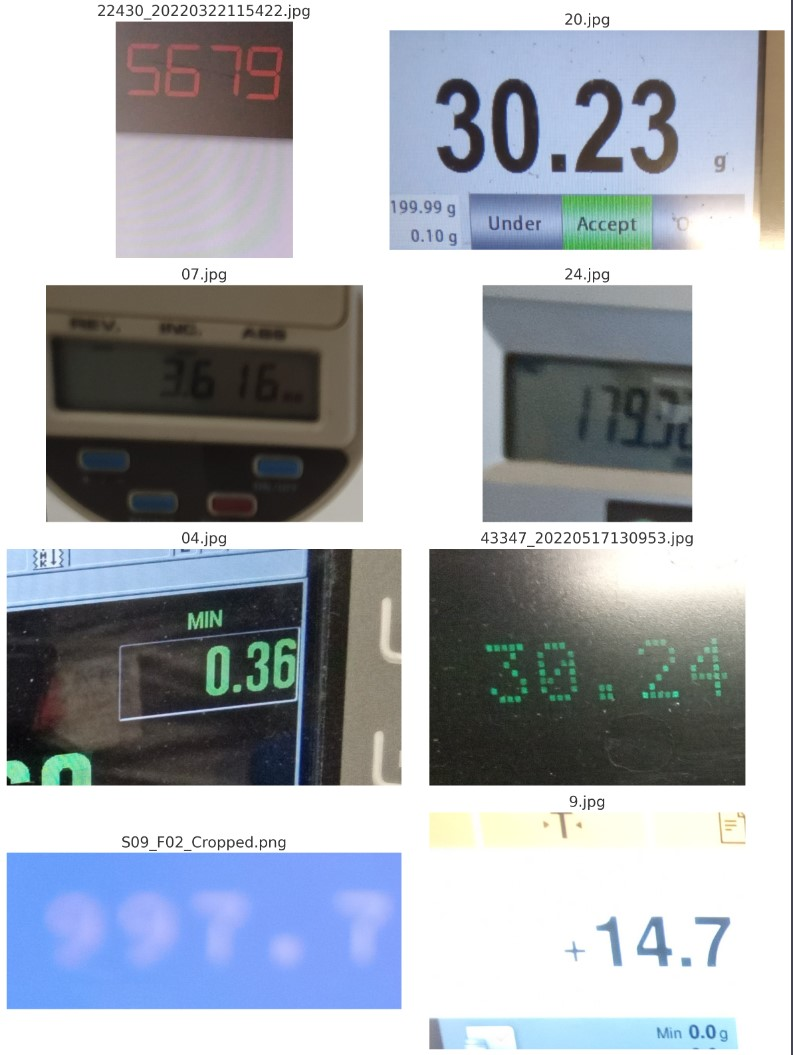
\includegraphics[width=0.6\textwidth]{Figures/discussion/unread_images.jpg}
    \caption[Selection of Unread Images]{Selection of Unread Images}
    \label{fig:Selection of Unread Images}
\end{figure}

Recognizing this challenge is crucial, as it emphasizes the importance of image quality in achieving optimal outcomes. Future research might focus on developing methods to enhance the readability of such images, exploring pre-processing techniques, and optimizing camera positioning under ideal conditions. Proper testing of these placements can also play a pivotal role in mitigating the impact of image quality on results.

\subsection{Fourth Sprint - CRNN Model Analysis}
In addition to Tesseract, the study also evaluated the performance of Convolutional Recurrent Neural Network (CRNN) models as an OCR tool. At least one CRNN model was developed per image folder. The models were trained using fonts that closely resemble those in the image dataset pertaining to that folder. The CRNN models underperformed in comparison to Tesseract with this author attributing this to the following reasons:

\begin{enumerate}
    \item \textbf{Partial Accuracy in Sensor Readings:} Some models were able to make accurate predictions of specific digits, such as 2, 3, 4, 5, 7, and 9. However, it sometimes misinterpreted the digit 8 as 6. This would return an ''incorrect'' prediction, even though the model was able to correctly identify the majority of the digits in the sensor reading.

    \item \textbf{Challenges in Digit Segmentation during Pre-processing:} A pivotal step in CRNN pre-processing is the segmentation of individual digits for prediction. Especially in noisy images, this step becomes arduous. Noise can obfuscate the model's ability to discern and correctly segment digits, influencing overall prediction accuracy.

    \item \textbf{Overfitting:} With their deep architectures, CRNNs can be prone to overfitting, especially when trained on a limited dataset or if the font type selected was not identical to the digits on the sensor readings.

    \item \textbf{Insufficient Training Data:} CRNNs often require a significant amount of labelled training data for optimal performance. The limited dataset lead to poor generalization in some instances.

    \item \textbf{Complexity:} The interplay between CNN and RNN layers can make CRNNs computationally intensive, affecting training and fine-tuning durations.


    \item \textbf{Alignment Issues:} In tasks like Optical Character Recognition (OCR), there can be misalignment between the predicted sequence and the ground truth, leading to discrepancies in results.

    \item \textbf{Lack of Invariance:} If not trained on a diverse set of data, CRNNs might not handle variations like rotations, scaling's, or other transformations effectively. Variations were introduced into the training data, however it is likely that these variations were not sufficient to ensure invariance.

\end{enumerate}

\subsection{Image Pre-processing Techniques}

Image pre-processing is instrumental in bridging the gap between raw data and actionable insights in the domain of machine learning. By refining the input data, these techniques set the stage for models to deliver optimal performance. Here, we dissect the significance and impact of various pre-processing techniques employed across different image folders:

\begin{itemize}
    \item \textbf{Grayscale Conversion:} This step, indispensable for Tesseract, simplifies the image by eliminating colour variations by converting three colour channels (RGB) to one single channel, allowing the algorithm to focus solely on structural features.

    \item \textbf{Resizing:} The dimensions of an image play a pivotal role in determining Tesseract's performance. By systematically testing a range of sizes, the optimal dimensions that yielded the highest recognition accuracy were identified.

    \item \textbf{Thresholding Techniques:} By binarizing the image, thresholding techniques accentuate the contrast between the text and the background, facilitating clearer text recognition.

    \item \textbf{Denoising:} Real-world images often come with their fair share of noise. Denoising techniques were employed to cleanse the images, making them more palatable for the subsequent processing steps.

    \item \textbf{Deblurring:} Motion blurs or out-of-focus images can obfuscate details. Deblurring techniques were harnessed to sharpen the images, ensuring that the text details remained discernible.

    \item \textbf{Red Mask} A tailored red mask was developed for Image Folder A, elevating the model's accuracy from an initial 1\% to a commendable 47.42\%.

    \item \textbf{Green Mask:} The introduction of a green mask filter significantly bolstered the accuracy of predictions. In the case of Image Folder E, while the second iteration registered a 20\% accuracy, the application of the green mask in a later sprint escalated this figure to 100\%. Similarly, the accuracy for Image Folder F experienced an uptick upon the integration of the green mask filter.

\end{itemize}

The key takeaway from these experiments is that meticulous and tailored pre-processing can have a significant impact on performance. By accounting for the unique characteristics of each dataset, these techniques can not only improve performance but also reveal the potential of data refinement to transform results.

\subsection{Comparative Analysis using CRNN Models}

The results show that the effectiveness of Tesseract and CRNN depends on the type of images and the pre-processing techniques used. Tesseract performed better in some folders, while CRNN performed better in others. This variability highlights the importance of understanding the dataset's characteristics and tailoring pre-processing techniques accordingly. Future research could focus on improving these techniques or developing hybrid approaches that combine the strengths of both methods.

\newpage

\section{Challenges and Limitations}

The study, while providing valuable insights, was not without its challenges and limitations. These constraints, detailed below, offer avenues for future research and refinement.

\begin{enumerate}
    \item \textbf{Data Variability:} The disparate characteristics across different image folders influenced the performance of both Tesseract and CRNN. Achieving consistent accuracy across folders with varying image quality and content was challenging.

    \item \textbf{Image Quality:} Some images, inherently noisy, blurred, or of low resolution, impeded the recognition algorithms' accuracy.

    \item \textbf{Segmentation Issues:} Proper digit segmentation, especially in the presence of image noise, posed significant challenges. Noise often obfuscated the differentiation and correct segmentation of digits.

    \item \textbf{Misinterpretation of Digits:} Specific digits, like 8 being recognized as 6, were consistently misinterpreted, indicating potential pitfalls in the recognition process.

    \item \textbf{Pre-processing Limitations:} The efficacy of pre-processing techniques varied. Techniques like the green mask might excel for one folder but falter for another.

    \item \textbf{Computational Constraints:} The deep architectures of CRNNs demanded substantial computational resources, constraining extensive hyperparameter tuning or exploration of intricate models.

    \item \textbf{External Factors:} Aspects like lighting conditions, shadows, and potential background interference during the initial image capture could have affected recognition accuracy.

    \item \textbf{Overfitting:} The risk of overfitting, especially pertinent given the complexity of CRNNs, was a concern, particularly as the training dataset lacked diversity.

    \item \textbf{Training Data Limitations:} A non-comprehensive training dataset, missing certain image variations, compromised the model's generalization capabilities.

    \item \textbf{Algorithm Limitations:} Both Tesseract and CRNN, while robust, come with inherent limitations. Tesseract had issues with specific fonts or styles, whereas CRNN faces challenges with sequence length variability. This lead to the need for tailored pre-processing techniques such as digit segmentation.
\end{enumerate}

\subsection{Analysis of OpenCV}

\textbf{OpenCV} is a powerful and versatile tool for computer vision tasks. It has a wide range of functionalities, from basic image pre-processing to advanced techniques. This makes it a good choice for a wide variety of projects.

However, OpenCV's extensive feature set was a drawback at the beginning of this project. The learning curve was steep, and it was difficult to know where to start. Additionally, OpenCV is not specifically designed for deep learning-based vision applications. For these tasks, specialized frameworks like \textbf{TensorFlow} or \textbf{PyTorch} may be a better choice. OpenCV was chosen for this project

\subsubsection{Detailed Breakdown of OpenCV's Strengths and Weaknesses}

\textbf{Strengths:}
\begin{itemize}
    \item \textit{Wide range of functionalities}: OpenCV has a wide range of functions for image processing, object detection, and machine learning. This makes it a good choice for a variety of projects.
    \item \textit{Seamless integration with other libraries}: OpenCV can be seamlessly integrated with other popular libraries, such as \textbf{NumPy} and \textbf{Python Imaging Library (PIL)}. This makes it easy to build complex applications.
    \item \textit{Performance}: OpenCV is written in C/C++, which makes it fast and efficient.
    \item \textit{Open source}: OpenCV is open source, which means it is free to use and modify.
\end{itemize}

\textbf{Weaknesses:}
\begin{itemize}
    \item \textit{Steep learning curve}: OpenCV's extensive feature set can make it difficult to learn.
    \item \textit{Not specifically designed for deep learning}: OpenCV is not specifically designed for deep learning-based vision applications. For these tasks, specialized frameworks like \textbf{TensorFlow} or \textbf{PyTorch} may be a better choice.
    \item \textit{Documentation}: OpenCV's documentation can be outdated and difficult to understand.
\end{itemize}

\subsection{Analysis of Tesseract}
Tesseract is a powerful and versatile open-source OCR tool. It has been evolving for decades and is now one of the leading OCR tools available. During this project, Tesseract yielded optimal results only when specific pre-processing steps were applied to the images; it did not excel as a generic tool without tailored interventions.

However, like all tools, Tesseract has its strengths and weaknesses. It is most accurate when the input images are of high quality and the document layout is simple. In cases where the images are low quality or the document layout is complex, Tesseract was not be able to accurately recognize the text.


\newpage

\section{Implications and Applications}

The results of this research not only provide insights into the intricacies of optical character recognition but also pave the way for tangible advancements in various application domains.

\subsection{Contributions to the Field of OCR}

The comparison of Tesseract and CRNN highlights their respective strengths and limitations, guiding researchers in tool selection based on dataset characteristics. The challenges identified can also direct future OCR improvements.

\subsection{Reading Sensor Data}
The ability to accurately read sensor data has vast implications. Automated and accurate sensor data readings can lead to:
\begin{itemize}
    \item Improved monitoring and reporting in industrial settings.
    \item Enhanced data integrity, minimizing human-induced errors.
    \item Efficient real-time tracking, leading to timely decision-making.
    \item Cost savings by reducing manual monitoring efforts.
\end{itemize}

\subsection{Real-world Applications and Benefits}
Beyond sensor data reading, the findings of this research can be extrapolated to various real-world scenarios:
\begin{itemize}
    \item \textbf{Healthcare:} Automated reading of medical tests, patient data, or prescription labels.
    \item \textbf{Logistics:} Recognizing and sorting packages based on labels or addresses.
\end{itemize}
Each of these applications not only enhances efficiency but also contributes to a more streamlined and error-free operational environment.

\section{Conclusions}

This research embarked on a journey to delve deep into the intricacies of optical character recognition, specifically comparing the prowess of Tesseract and CRNN. Through experimentation and analysis across diverse image folders, several pivotal insights were unearthed:

\begin{itemize}
    \item The efficacy of both Tesseract and CRNN is heavily influenced by the nature of the images and the pre-processing techniques employed. While Tesseract showcased superior performance in certain folders, CRNN emerged as the preferred choice in others.
    \item Image quality, manifested through challenges like light reflection, blurriness, and skewness, plays a cardinal role in determining recognition accuracy. Addressing these challenges through tailored camera recommendations and advanced pre-processing can significantly bolster recognition rates.
    \item The study underscored the transformative potential of bespoke data refinement. Treating each dataset with its unique idiosyncrasies in mind can pave the way for substantial improvements in recognition accuracy.
\end{itemize}

This author believes this research holds some significance. As the digital world continues to expand, the demand for efficient and accurate OCR systems is escalating. By highlighting the strengths, limitations, and potential areas of improvement for both Tesseract and CRNN, this study provides a roadmap for future endeavours in the field. The insights gleaned not only contribute to the academic corpus of OCR but also have tangible implications for real-world applications, from reading sensor data in industrial setups to streamlining operations in sectors like healthcare, retail, and logistics.

In conclusion, while there remain avenues for further exploration and refinement, this research stands as a testament to the strides made in enhancing OCR performance and the promising horizons that lie ahead.



\section{Recommendations and Future Work}

\subsection{Camera Recommendations for Enhanced Image Capture}

The quality of captured images plays an important role in determining the efficacy of subsequent processing and analysis. To address challenges like light reflection, blurriness, and skewness, the following camera recommendations are proposed:

\begin{itemize}
    \item \textbf{Optimal Lighting:} Ensure a uniform lighting environment during image capture. Avoid placing sensors under direct light to prevent reflections. The use of diffused lighting or soft-boxes can help mitigate harsh glares and reflections.

    \item \textbf{Camera Stability:} To minimize image blurriness, employ tripods or stable platforms for camera mounting, ensuring a steady capture process.

    \item \textbf{Adjust Focus:} Regular camera focus calibration is crucial. Cameras equipped with an adaptive auto-focus feature can be particularly advantageous for varying capture distances.

    \item \textbf{Angle Consistency:} To curtail skewed image captures, position the camera perpendicular to the sensor. Adjustable mounts or stands can facilitate precise angle alignments.

    \item \textbf{Define Region of Interest (ROI):} Utilize cameras that allow for ROI definition. By delineating the ROI, cameras can prioritize and focus on the specified area, especially beneficial in environments with potential visual noise or distractions.

    \item \textbf{Image Resolution:} Opt for high-resolution cameras to discern finer details. Even if resizing becomes necessary during post-processing, higher resolution images offer a more detailed foundation.

    \item \textbf{Lens Choice:} Lenses with anti-reflective coatings can further diminish glare and undesired reflections.

    \item \textbf{Background Contrast:} A contrasting background relative to the sensor can significantly aid in distinguishing the sensor during subsequent image processing tasks.
\end{itemize}

Adhering to these recommendations can markedly enhance image capture quality, paving the way for more accurate and efficient data analysis. Such guidelines serve as a bedrock for future research, underscoring the importance of pristine initial data capture.

\subsection{Future Work}

As the field of OCR continues its evolutionary trajectory, myriad promising avenues beckon exploration. Highlighted below are some of the compelling avenues for future research:

\begin{itemize}
    \item \textbf{Exploration of Other Neural Network Architectures:} Delving into architectures beyond the conventional, like Transformer-based models or Capsule Networks, holds promise. Recognized for their efficacy in various sequence recognition tasks, adapting these architectures for OCR could herald significant advancements.

    \item \textbf{Real-world Deployment and Scalability:} The litmus test for any OCR system lies in real-world deployment. This necessitates a deep dive into factors encompassing scalability, computational efficiency, and a design that is user-centric.

    \item \textbf{Integration with Augmented Reality:} Melding OCR with augmented reality (AR) can usher in real-time text recognition within a live augmented environment, potentially enhancing user experiences and diversifying OCR applications.

    \item \textbf{Semi-supervised and Unsupervised Learning:} Given the labour-intensive annotation requirements of data, semi-supervised and unsupervised learning paradigms could be pivotal. Harnessing vast unlabelled data pools can expedite the journey towards more refined OCR systems.

    \item \textbf{Feedback Loop for Continuous Learning:} Infusing OCR systems with a user feedback loop can be transformative. This mechanism, allowing users to rectify inaccuracies, ensures the system's continuous learning and refinement.

    \item \textbf{Security and Privacy:} With OCR systems processing increasingly sensitive data, underpinning them with robust security and privacy measures becomes non-negotiable. This calls for advanced encryption methodologies and cutting-edge anonymization techniques.

    \item \textbf{Customizable OCR Systems:} Tailoring OCR systems to individual user needs and diverse applications can ensure their broader relevance. Systems, when designed with customization or fine-tuning capabilities, can cater to a gamut of specific requirements.
\end{itemize}

These facets merely scratch the surface of the vast expanse of potential research directions in OCR. Fuelled by relentless innovation, the horizon looks promising with OCR systems poised to be more precise, agile, and adaptable, catalysing a plethora of novel applications.

The journey of this research is a reflection of the evolving nature of OCR, and while conclusions have been drawn, it also marks the beginning of numerous possibilities and questions yet to be explored.


